\documentclass[
12pt, paper=a4,  listof=totocnumbered, % lists are also included in table of contents
, % Don't add a period at the end of a chapter number
]{scrreprt}

\usepackage{chngcntr}
    \counterwithout{footnote}{chapter}
    \counterwithout{figure}{chapter}

% get custom bibliography style working without prepending [brackets]
\usepackage{natbib}

%\setcitestyle{aysep={}} % remove comma as delimiter 

% breaks line at hyphens (resolves formatting issues in bibliography)
\usepackage[hyphens]{url}

% if you insist on Arial... then uncomment the following
\usepackage{helvet}
\renewcommand{\familydefault}{\sfdefault}

\usepackage[left=2.5cm,right=2.5cm,top=2.5cm,bottom=2.5cm]{geometry} % margins
%\addtolength{\footskip}{-0.7cm}% foot larger by 0,7 cm  (Raises the page number)


%\usepackage[onehalfspacing]{setspace} % line space 1,5
\usepackage[doublespacing]{setspace}
%\doublespacing

%\setlength{\parindent}{12pt} % Indent at start of paragraphs  6pt

\usepackage[utf8]{inputenc} %UTF-8 to encode many characters => for many characters, you can just input the character and avoid a macro

\usepackage[english]{babel} % english hyphenations
%\usepackage[T1]{fontenc} %wichtig für Trennung von Wörtern mit Umlauten
\usepackage{microtype} % align margins

% for multi line comments
\usepackage{comment}

\usepackage{graphicx} % import graphics
\usepackage{placeins}% places the graphics within text

% Abbreviation's directory
% printonlyused - only if used
% withpage - the first occurrence's page number is listed too
\usepackage[withpage]{acronym}

% for tables
\usepackage{longtable}
\usepackage[table]{xcolor}
\usepackage{multirow}


\usepackage[hidelinks]{hyperref} %https://tex.stackexchange.com/questions/823/remove-ugly-borders-around-clickable-cross-references-and-hyperlinks

\newcolumntype{P}[1]{>{\endgraf\vspace*{-\baselineskip}}p{#1}}
\usepackage{etoolbox}
\makeatletter
\patchcmd{\chapter}{\if@openright\cleardoublepage\else\clearpage\fi}{}{}{}
\makeatother

\usepackage{enumerate} % http://ctan.org/pkg/enumerate

%for chapter spaces
\begin{document}

%\renewcommand{\thechapter}{\Roman{chapter}}
%TITELBLATT:!!!!!!!!!!!!!!!!!!!!!!!!!!!!!!!!!!!!!!!!!!!!!!!!!!!!!!!!!!!!!!!!!!!!!!!!!!!!!!!!!!!!!!!!!!!!!

\label{titlePage}
\begin{figure}[h]
\centering

\includegraphics[width=0.50\textwidth]{pics/logo.pdf}
\end{figure}
\FloatBarrier

\begin{Large} 
\begin{center}
MSc. Thesis
\end{center}
\end{Large} 

\vspace*{5mm}

\begin{large} 
\begin{center}
University of Essex
\end{center}
\end{large} 

\begin{large} 
\begin{center}
Study Branch: MSc. Cyber Security
\end{center}
\end{large}



\begin{Large} 
\begin{center}
\textbf{OpenID Connect Protocol's Security Risk Analysis in Cloud Based Applications}
\end{center}
\end{Large}

\vspace*{5mm}

\begin{large} 
\begin{center}
Advisors: Dr. Sabeen Tahir and Dr. Nkaepe Olaniyi
\end{center}

\end{large} 

\begin{center}
{\today}
\end{center}

\pagestyle{empty} % no page numbering on the cover



\renewcommand{\thechapter}{\Roman{chapter}}

\pagestyle{plain}

\pagenumbering{Roman} %the intro is counted with roman numbers
\setcounter{page}{2} %starting with page 2 (page 1 is the titel)

\tableofcontents %table of contents
\listoffigures %List of figures
\listoftables %list of tables

% Abbreviations list
\renewcommand\refname{Abbreviations} \chapter{Abbreviations}
% The abbreviations list should contain all abbreviations that are not common-knowledge.
\begin{acronym}[DSRM] % the longest abbreviation here (for layout)

    \setlength {\itemsep}{-\parsep} % geringerer Zeilenabstand    	 
    \acro{DSRM}{Design and Research Methodology}
    \acro{DFD}{Data Flow Diagram}
    \acro{GDPR}{General Data Protection Regulation}
    \acro{IdM}{Identity Management}
    \acro{JWT}{JSON Web Token}
    \acro{MCC}{Mobile Cloud Computing}
    \acro{OIDC}{OpenID Connect}
    \acro{PKCE}{Proof Key for Code Exchange}
    \acro{SDLC}{Software Development Life Cycle}
    \acro{SPA}{Single Page Application}

    

\end{acronym}



% Acronyms should be made hyperreffed the first time they appear in text with
% \ac{CI}  

\renewcommand{\thechapter}{\arabic{chapter}} %Count chapters with arabic numbers and not roman numbers
\setcounter{chapter}{0} %Reset chapter counter
\pagenumbering{arabic}

\chapter{Introduction}
\section{Background}
In the era of digitalisation, an immense transformation is commencing where day-to-day services such as shopping, communicating with people, visiting university courses, and also critical services like accessing financial services, accessing health services, running powerplants, managing traffic, and managing public services are moving digital \citep{intro_cloud_critical_infra}. This transformation is fundamentally changing the traditional analogue methods and replacing them with continual innovations, enhancing efficiency and improving user experience by providing a digital platform in the form of different applications/software hosted in the Cloud. For example, in 2023, the German administration created a cloud strategy plan with the German Administration Cloud Strategy (DVS) to incorporate, strengthen and improve the status quo of digitalisation in the public sector \citep{german_gov_cloud_plan}. Such moves are not isolated to a single country and signals a move towards cloud and digitalisation to shape the new world. \newline

As this modernization reshapes the business landscape, there is a need to ensure that only legitimate users gain access to sensitive data and systems to safeguard personal data as well as unauthorized breaches, which can lead to loss of intellectual property, violation of laws and regulations and disruption to public services \citep{critical_infra_reason}. Therefore, authentication and authorisation are fundamental concepts in cybersecurity, crucial for safeguarding digital resources and ensuring proper access control. \newline

Authentication is the process of verifying the identity of a user or an online service using credentials like passwords, biometrics, or tokens \citep{authetication_intro}. On the other hand, authorization determines the permissions or defines the granular access levels a user can execute, ensuring only the actions one is entitled to are used \citep{Gollmann2021-at}. Having both mechanisms to secure systems and avoid sensitive information and unauthorised access is crucial. Especially now, where the cloud-computing industry is booming, many services are easily accessible to a larger group of people, as it is easier to run and create different applications and simultaneously give attackers more systems to compromise.\newline

In addition to the benefits that cloud computing provides, such as easy accessibility and quicker setup of applications, it has also introduced new challenges. In particular, the shared responsibility model of the Cloud, where the cloud provider and the client both have specific responsibilities to secure the system \citep{shared_principal}. This complication increases the attack surfaces to exploit as different errors and misconfiguration could make the system more vulnerable. Therefore, the combination of authentication and authorization for applications running in the cloud has gained significance. 


\section{Problem Statement}
Cloud computing and applications needing authorisation and authentication capabilities are synonymous, as many systems are rapidly moving to this environment. This way of operating business has been revolutionary, as it leverages a group of distributed systems located on remote servers hosted on the internet. The main benefit of using such a distributed network of readily available systems is also the main challenge for securing the system \citep{Alouffi2021-yh}. Especially when it comes to authentication and authorisation, it can be very critical as the vulnerabilities in this area will lead to unauthorised access and data leaks, which can be very costly; Statista reported in 2023 that the average cost of such a data breach is about 4.45 million US dollars \citep{statista_data_breach}. Therefore, this thesis will investigate the security risks associated with authentication and authorisation protocols in a cloud-based application using the Open ID connect protocol (OIDC) in the cloud, as OIDC is one of the most widely used protocols for Identity Management (IdM), which supports different modes such as mobile applications, machine-to-machine, and Single Sign-On (SSO) \citep{oidc_popular}.

\section{Research Question and Objectives}\label{sec:objectives}
\textbf{\textit{RQ1: What are the primary security concerns of the OpenID Connect protocol when used in a cloud-based application?}.}

The primary aim of the RQ1 is to systematically analyse the security risks associated with implementing and using the OIDC protocol in cloud-based applications by identifying common vulnerabilities, assessing their impact on the overall security of these applications, and proposing effective mitigation strategies. Pursuing this aim, the thesis has the following objectives and goals:

\begin{enumerate}
  \item Identify Common Security Risks - Describe the most prevalent security risks of OIDC Connect protocols when used with cloud applications.
  \item Conduct Risk assessment  - Conduct a risk assessment of an Identity provider application, using threat modelling and mitigations for identified risks.
  \item Design and develop Prototype - A prototype containing the investigation's main findings and essential features.
\end{enumerate}


\section{Research Methodology}
The research will adhere to the Design Science Research Methodology (DSRM) for Information Systems Research. The DSRM is a robust framework for studying, creating, and evaluating IT artefacts. It is a suitable choice for this master thesis, which aims to design and develop artefacts for the OIDC protocol in a cloud-based application. This methodology is selected because it provides specific guidelines tailored for creating and implementing systems essential for conducting Design Science (DS) research in information systems \citep{dsrm}.

The DSRM framework encompasses six steps: problem identification, definition of objectives, design and development, evaluation, demonstration, and communication \citep{dsrm}. These steps align seamlessly with the goals of this research. The primary aim of this project is to identify and evaluate potential risks associated with the OIDC protocol in a cloud-based application. Based on the insights gained from this evaluation, the project will proceed to design, create, and rigorously test a prototype. This approach ensures a structured and methodical examination of the OIDC protocol’s vulnerabilities and mitigations, thus aligning with the objectives outlined in section \ref{sec:objectives}.

In detail, the process begins with problem identification, where the specific security challenges and vulnerabilities of the OIDC protocol in cloud environments are identified. Following this, the objectives are defined, and clear goals for the research are set, particularly regarding risk assessment and artefact development. The design and development phase involves creating security artefacts, such as threat models based on the discovered risks.

The evaluation phase will assess these artefacts through various code and security testing methods to ensure their effectiveness and reliability. Demonstration involves showcasing the developed prototypes in practical scenarios to validate their functionality. Finally, the communication phase focuses on disseminating the findings and methodologies through comprehensive documentation and presentations, ensuring that the research contributes valuable insights to the broader field of information systems security.

By adhering to this structured methodology, the research addresses the immediate goals of evaluating and mitigating some risks associated with the OIDC. It provides a qualitative analysis that can inform future developments in the field. DSRM ensures that each research phase is meticulously planned and executed, ultimately leading to the development of robust security solutions for this use case.



\chapter{Literature Review}

This chapter aims to critically analyze the existing literature on cloud computing and OpenID Connect (OIDC) protocols, focusing on identifying security risks and highlighting gaps in current research. By examining these areas, the chapter will provide a foundation for understanding the complexities and challenges of securing cloud applications using OIDC. It will also offer an overview of cloud computing and OIDC to contextualize their interrelated roles in modern technology environments.

\section{Overview of Cloud Computing}
Cloud computing is a service model that provides on-demand access to a wide range of computing resources via the internet, including servers, storage, databases, networking, software, and analytics \citep{rashid2019cloud}. These services are designed to be easily manageable and deployable, often requiring minimal effort from the user. For example, users can quickly launch servers using a web browser through Cloud Service Providers (CSPs) such as AWS, Google Cloud and Microsoft Azure. 

Beyond simply running applications, cloud computing is evolving with new concepts like mobile cloud computing. One such concept is mobile cloud computing (MCC), a popular architectural model that integrates cloud computing with mobile technology. This model allows mobile devices to leverage the extra power and storage capacity of cloud-based resources, helping to overcome mobile hardware limitations \citep{mcc}. However, such models also pose latency, data security, and network dependency challenges. Addressing these issues requires robust network infrastructure, efficient data encryption, and effective management strategies to ensure privacy and reliability.

\section{Deployment Models}
The cloud offers different deployment models, each with varying levels of complexity and control, allowing consumers to choose the best fit for their needs, typically classified into public, private, hybrid, and community clouds. Security is a critical aspect that influences the choice of a deployment model; see Table \ref{table:cloud_comp} for a comparison. 
\begin{itemize}
    \item  \textbf{Public Cloud} - This model is the most used method to deploy applications in the cloud, preferred for running web applications, file sharing, and non-critical systems needed top-level privacy \citep{cloudmodel}. Public cloud services are also considered more cost-effective as the consumers can pay as they go. Public cloud providers often have multiple data centres worldwide, offering redundancy and high availability. This ensures that services remain available even if one data centre experiences issues. Public cloud providers also offer a range of managed services, such as databases, machine learning tools, and analytics platforms, which allow organizations to leverage advanced technologies without maintaining the underlying infrastructure. 
    
    While public clouds offer numerous benefits, security remains a primary concern. Key security considerations include data privacy and ensuring that sensitive data is encrypted and managed securely. Organizations must also ensure that their use of the public cloud complies with industry regulations and standards. Properly managing access controls and user permissions is essential to protect resources. Businesses should also consider strategies to avoid vendor lock-in to maintain flexibility and control  \citep{cloudmodel}.
    
    \item  \textbf{Private Cloud} - A Private cloud is a deployment model dedicated to a single consumer who does not share resources with multiple users to maintain a high level of privacy. The organization manages its resources and who has access to it. Some private clouds are also hosted in a local data centre to have greater infrastructure separation \citep{cloudmodel}. The principal characteristic of this model is to provide exclusive access to the resources only to the organisation, ensuring more significant levels of privacy and security. 
    
    However, the greater flexibility to customize the private cloud environment to meet specific business needs and performance comes with its challenges. Building and maintaining a private cloud can be more expensive than public cloud services due to the need for dedicated hardware and skilled IT staff. Managing a private cloud environment requires expertise and can be complex, particularly for organizations with limited IT resources. Additionally, private clouds may have limitations in scalability, depending on the organization's infrastructure and resources \citep{private_cloud}. \newline
    \item  \textbf{Hybrid Cloud} - As the name suggests, the hybrid cloud model combines both public and private clouds to achieve the best of both worlds and create a flexible, scalable computing infrastructure with the desired amount of control for critical assets. This model allows organizations to leverage the benefits of both cloud types while addressing specific business needs related to security, performance, and cost efficiency. By integrating public and private clouds, organizations can dynamically manage workloads, optimize resource usage, and improve business agility \citep{cloudmodel}.

    While the hybrid cloud offers numerous advantages, it also presents particular challenges. Managing and integrating multiple cloud environments can be complex and require robust IT expertise and tools. Ensuring seamless connectivity and interoperability between public and private clouds is critical to achieving the desired benefits. Organizations must also address security and compliance issues across both environments, implementing consistent policies and procedures to protect data and maintain regulatory compliance that requires additional tools and expertise, increasing the costs for running such a model \citep{hybrid_model}.
   
    \item  \textbf{Community Cloud} - A community cloud is a cloud deployment model where several organizations share the infrastructure with common interests, goals, or regulatory requirements. This model is designed to meet the specific needs of a particular community, such as industry groups, government agencies, or academic institutions. The community cloud offers a balanced approach, combining the shared resource benefits of a public cloud with the enhanced security and compliance controls of a private cloud. Organizations within the community share the costs, making it a cost-effective solution \citep{cloudmodel}.
\end{itemize}

\begingroup
\centering
\setlength{\tabcolsep}{6.5pt} % Default value: 6pt
\begin{longtable}{|p{2cm}| p{3cm} |p{3cm} |p{3cm}|p{3cm}|}
\caption{Cloud Deployment model comparison}
    \label{table:cloud_comp}
\hline
\rowcolor{grey!15}
\textbf{Feature} & \textbf{Private Cloud} & \textbf{Public Cloud} & \textbf{Hybrid Cloud} & \textbf{Community Cloud} \\
\hline
\endfirsthead
\hline
\rowcolor{grey!15}
\textbf{Feature} & \textbf{Private Cloud} & \textbf{Public Cloud} & \textbf{Hybrid Cloud} & \textbf{Community Cloud} \\
\hline
\endhead
\hline
\endfoot
\hline
\endlastfoot

Cost & Higher initial investment; lower ongoing costs if managed well. & Typically lower initial investment; pay-as-you-go model. & Mix of both; can be cost-effective if managed properly. & Costs shared among organizations; generally lower than private cloud. \\
\hline
Security & High; dedicated infrastructure, more control. & Variable; depends on the provider’s security measures. & Variable; depends on integration and management. & Moderate; shared infrastructure with similar organizations. \\
\hline
Compliance & Easier to meet specific regulatory requirements due to dedicated resources. & May meet general compliance standards; might require additional controls for specific needs. & Can meet compliance if managed properly with both environments. & Often easier to meet compliance for shared needs of community members. \\
\hline
Scalability & Limited by physical resources; scaling can be expensive. & Highly scalable; can quickly adjust resources based on demand. & Highly scalable; combines public cloud's scalability with private cloud’s control. & Limited scalability; constrained by shared resources within the community. \\
\hline
Ownership & Owned and operated by the organization or a third party dedicated to the organization. & Owned and operated by the cloud service provider. & Ownership is shared between private and public components. & Owned and operated by the community or a third party dedicated to the community. \\
\hline
Use Cases & Suitable for sensitive data and mission-critical applications. & Ideal for general-purpose applications, web hosting, and businesses with variable needs. & Good for organizations needing a mix of private and public resources, such as data privacy and scalable resources. & Best for organizations with common interests or regulatory requirements, such as government agencies or academic institutions. \\
\hline
Control & High; full control over infrastructure and data. & Limited; control is restricted to what the provider offers. & Variable; control over private components is high but limited over public components. & Moderate; control is shared with other community members and governed by shared policies. \\
\hline
Reliability & High if well-managed; depends on infrastructure and management practices. & Generally high; providers offer redundancy and failover solutions. & High; combines the reliability of private and public cloud components. & Generally reliable; depends on the community's infrastructure and management. \\
\hline
\end{longtable}
\endgroup

\section{Risks}
\begin{itemize}
    \item \textbf{Access Control In the Cloud} - Access control in the cloud is critical to securing the system and sensitive data. However, managing the access control has risks, especially when the controls are misconfigured, as the cloud follows a shared responsibility for securing the systems between the customer and the cloud provider \citep{cloud_shared_resp}. Such misconfiguration of identity and access management (IAM) policies, weak authentication practices, and poor management for storing and rotating secret keys can lead to unauthorised access.  

    \item \textbf{Network Security } - Network security in cloud computing faces unique challenges that can compromise data and service integrity. One of the primary risks is insecure API endpoints, where attackers can exploit vulnerable APIs lacking proper authentication and encryption to gain unauthorized access to cloud resources, leading to data breaches and service disruption. Network security issues have a lot of commonalities with the traditional, like DDoS, Man-in-the-Middle (MitM)  and VM vulnerabilities, especially with cloud sharing infrastructure where the infrastructure is shared amongst many clients \citep{network_cloud}. If proper measures and configurations are not in place, attackers could move laterally across the cloud to infiltrate many systems and organisations simultaneously. 
    
    \item \textbf{Regulatory Compliance } - Cloud computing has added complexity as Cloud providers tend to be multi-regional, which presents significant challenges to organisations operating across different regions, and the areas are subject to strict requirements for data protection, security controls and data sovereignty. This risk, in particular, is not a security risk but rather a legal one, where not failure to comply with local laws and regulations such as HIPAA, GDPR, and PCI DSS could lead to financial and reputational damage \citep{legal_cloud_challenge}.
    
    \item \textbf{Malware on Mobile Cloud Computing } - Cloud computing has evolved from the traditional web application to being used for mobile, also known as Mobile Cloud Computing. Malware injection is a significant threat to MCC. Attackers can embed malicious code into legitimate mobile applications, leading to harmful activities such as stealing sensitive data or using cloud computing power for tasks like crypto mining, also known as cryptojacking \citep{cryptojacking}. The interconnected nature of cloud computing means that malware introduced into one device can potentially spread to other devices or services within the same cloud environment. For instance, if a cloud-based application becomes infected, all users accessing that application are at risk of having their data compromised. Once malware is injected, it can persistently attack the mobile device, extract valuable information, and send it back to the attacker, often without the user's knowledge.
    
    \item \textbf{Multi-tenancy} - Multi-tenancy security risks are very similar to the ones discussed in network security, as in a multi-tenant system, an organisation could use the same physical hardware as in a private deployment model. Such a system can lead to data leakages or unauthorised access if it is improperly configured or there are vulnerabilities in the cloud provider's software.   According to \citep{multi_tenancy_cloud_risk}, an attacker has a 40\% chance of allocating his VM besides the victims using tactics like side-channel attacks, which can be done with a moderate budget, making such attacks more probable.

\end{itemize}

\section{OpenID Connect Protocol}
OpenID Connect (OIDC) is a prevalent authentication layer based on the OAuth 2.0 protocol that provides a standardised way of authenticating and authorising users across web applications and apps \citep{oidc_intro}. OpenID Connect enables a secure sign-in experience and simplifies verifying user identities across various applications and platforms. This protocol allows applications to request and receive information about authenticated users from identity providers (IDPs), such as Google, Microsoft, and Facebook. The authentication process involves exchanging different types of tokens, usually in JSON Web Token (JWT) format, a widely adopted industry standard for exchanging information between two parties \citep{jwt}. These JWT tokens are then used as different kinds of Tokens, such as ID tokens, access tokens, and refresh tokens that contain claims or information about the user and the permissions they are allowed in the application and carry information about their sessions. Using these tokens, an application can authenticate and authorise users (Access Tokens), identify authenticated users (ID tokens) and provide a way to re-authenticate automatically without explicit login (Refresh tokens) \citep{oidc_tokens}; See Table \ref{table:oauth_terms} for more details. 

\begingroup
\centering
\setlength{\tabcolsep}{6.5pt} % Default value: 6pt
\begin{longtable}{|p{4cm}|p{10cm}|}
\caption{OpenID Connect Terms}
    \label{table:oauth_terms}
\hline
\rowcolor{grey!15}
\textbf{Term} & \textbf{Description} \\ 
\hline

\textbf{Client} & The app that wants to access some data. \\ \hline
\textbf{Resource server} & The resource that the client wants to access. This is generally an API or an app that contains some data. \\ \hline
\textbf{Resource owner} & The data owner on the server. \\ \hline
\textbf{Authorisation server} & The main server which issues the tokens after successful authentication.\\ \hline
\textbf{Grant Type} & This is an authorisation given to the client to access the data on the resource server, which represents the specific permission the client is allowed to have. Grant types include Authorisation Code, Implict, and Client Credentials \citep{adv_api_sec}.  \\ \hline
\textbf{Access token} & The token issued by the authorization server to get the resources from the resource server. \\ \hline
\textbf{Refresh token} & A token that is used to retrieve a new access token after expiry. \\ \hline
\textbf{ID token} & A token that contains user identity information which can verify the identity of the user. \\ \hline
\end{longtable}
\endgroup

\subsection{Flows}
OpenID Connect provides a means to authenticate users and allow them to access data using different kinds of tokens. Still, in the real world, various requirements exist for diverse types of application architecture, such as mobile, server-server, and single-page applications. The OpenID Connect protocol is designed with multiple flows that try to balance security and usability to accommodate designs encompassing different security requirements and technical limitations. For example, some flows prioritise security by not exposing sensitive tokens on the user end. On the other hand, user experience is more of a focus, making it less secure. 
\par
In the coming section, we will discuss these critical flows to understand their advantages and disadvantages. Understanding the OpenID Connect flows and their characteristics allows one to choose the most appropriate method for their specific application scenario to balance security, functionality, and user experience.



\subsubsection{Implict Flow}
The Implicit flow is the most straightforward authentication flow in the OpenID Connect protocol. It is designed to accommodate client-side applications or single-paged applications (SPAs) that run in a user's browser. This flow is primarily intended for scenarios where the client application cannot securely store client secrets, which is usually true for web applications, mobile apps, and SPAs. This method directly issues tokens like ID Tokens, access tokens, and refresh tokens after the user successfully authenticates as part of the response without additional network requests (See Figure \ref{fig:implicit_flow} for the flow). Such an authentication process is advantageous as the resource access does not need many steps and reduces latency, as the tokens are available after user authentication. 

\par
Despite the benefits of latency and simplicity, this approach comes with particular security risks, as the tokens are stored and handled directly in the client application or within the browser. This means that the tokens are vulnerable to various attacks. If the client applications are compromised and the tokens are exposed to the client application, this could lead to unauthorised access. The valuable tokens can be intercepted using different attacks, like man-in-the-middle attacks and cross-site Scripting, allowing the valid tokens to be replayed. While the Implicit Flow can provide quick and easy access to authentication tokens for client-side applications, it comes with significant security challenges. Developers must carefully consider these risks and apply appropriate security measures or, ideally, opt for more secure alternatives.

\begin{figure}[h!]
\centering
\caption{OIDC Implicit Flow}\label{fig:implicit_flow}
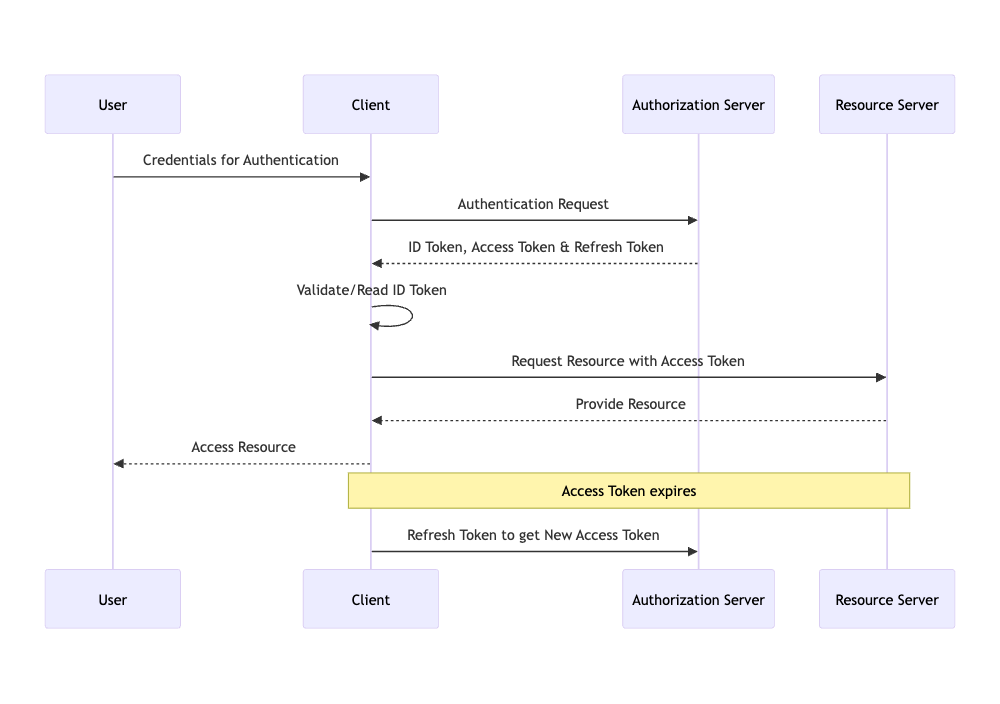
\includegraphics[width=\textwidth, height=320px]{pics/implicit_flow.png}
\end{figure}

\appendix 

% ---- Bibliography ----
%
% BibTeX users should specify bibliography style 
% References will then be sorted and formatted in the correct style.
%
 %\bibliographystyle{alpha}
\renewcommand{\bibname}{References}
\bibliographystyle{agsm}
\bibliography{biblio}

% formatting taken from http://tex.stackexchange.com/questions/149708/simple-list-of-abbreviations-manually
% sorting taken from http://www.latex-community.org/forum/viewtopic.php?f=44&t=16419

\end{document}
